
\documentclass[a4paper,11pt]{article}

\usepackage[plain]{fullpage}
\usepackage{graphicx}  %This enables the inclusion of pdf graphic files in figures
\usepackage{wrapfig}

\title{Lab Project, task 1}
\author{\O yvin Richardsen}
\date{ {\tt oyvinric@stud.ntnu.no }\\
TTM4120 Dependable Systems\\
\today}
 
\begin{document}
\maketitle

\section{Answers to the questions}

\subsection{
There are many distributed platforms that allow developers to implement distributed applications more easily.
Such platforms include Remote Procedure Call (RPC), CORBA and Java RMI. What are the main difficulties
in extending existing distributed platforms with fault tolerance, through the use of group communication?
}
\paragraph{}
\begin{itemize}
	\item Maintaining state consistency among the servers cooperating in the delivery of a service.
	\item Partitioning and merging the communication network, enabling one-to-many communication.
\end{itemize}

\subsection{
Java RMI is based on the client-server paradigm, while JaSoS combines this with the object group paradigm.
Explain the structuring of clients vs servers in the object group approach used by JaSoS.
}
\paragraph{}
The client communicates to a server group through a group proxy object that implements a service, and the client is thus not aware of the particular service implementation. A server group may serve many clients, and because of this object group concept with a proxy, a client may be served by many servers at the same time (typically the entire group).

\subsection{
What is needed before a client object can communicate with a server object group?
}
\paragraph{}
See previous answer. The communication is done through two proxies: the client proxy, and the server proxy. Both may be statically or dynamically created, and handles any messages to and from clients and servers. For any available service, the client proxy provides a service interface to the client, and must know about a server proxy in one or more object groups implementing the service. 

\subsection{
What is the task of the Partition-aware Group Membership Service (PGMS)?
}
\paragraph{}
The PGMS tracks group membership, both voluntary (joining and leaving the group) and involuntary (failures). Changes are reported to all members of the group through membership change messages, and each member then updates its group view. Order and some timeliness is important to maintain consistency across all servers.

\subsection{
Why should internal and external group invocations be distinguished?
}
\paragraph{}
IGMIs are performed by servers, while EGMIs are performed by clients. There are 3 reasons for this distintion:
\begin{itemize}
	\item \textit{Visibility:} Clients should only have access to a "public interface", and not the methods used for implementing the service. 
	\item \textit{Transparency:} Clients do not need to know that they are invoking a method on a group rather than a single server, but servers may need to invoke methods on each of the servers in a group.
	\item \textit{Efficiency:} Identical standards for IMGI and EMGI would require clients to become members of a group, reducing the scalability of the system.
\end{itemize}

\subsection{
What are the different Reliability levels are provided by Spread for message delivery. Which level is used by
JaSoS and why?
}
\paragraph{}
JaSoS uses the reliability level Safe, in order to guarantee that messages are delivered either to all recipients, or none of them.
\begin{itemize}
	\item \textit{Unreliable:} Message may be dropped or lost.
	\item \textit{Reliable:} Message will be delivered to all recipients.
	\item \textit{Safe:} The message will only be delivered to a recipient if the daemon that recipient is connected to knows that all Spread daemons have the message.
\end{itemize}

\subsection{
What is the default invocation semantics for External Group Method Invocations in JaSoS and how can it be
changed?
}
\paragraph{}
The default invocation semantics for JaSoS is anycast, but we can change this with Java Annotations (e.g. @Multicast).

\subsection{
Explain the problem with allowing several concurrent views.
}
\paragraph{}
When there are several object groups implementing the same service, state updates may cause inconsistencies, which could potentially damage the application.

\subsection{
The availability-consistency tradeoff relates to the semantics of a Group Communication System (GCS). Explain
the difference between a primary component partitioning GCS and a partitionable GCS, and which tradeoffs
are made with these two variants.
}
\paragraph{}
The main difference is that with the primary-partition approach, only servers in a primary partition may serve requests, while in a partition-aware approach, the application knows about other partitions, and may thus request the service from any of these partitions.
\begin{itemize}
	\item \textit{Primary-partition approach:} Strong consistency, low availability. Easy to maintain a single, shared state, but servers outside primary partitions cannot serve requests. This approach makes fault-tolerant application development simpler, but does not allow for exploiting application semantics in order to improve availability.
	\item \textit{Partition-aware approach:} High availability, loose consistency. Partitions evolve independently, which may cause inconsistency, but servers in any partition can serve requests. This is a more complex approach, but allows for adaptive applications, improving availability (but possibly reducing QoS).
\end{itemize}

\subsection{
Give the properties of the State Merging Service (SMS) and explain their importance.
}
\paragraph{}
\begin{itemize}
	\item Full information exchange: When multiple partitions merge into one, every server must receive the full state information of all the servers in the other partitions (realized by a one-round distribution scheme).
	\item Every server must be able to act as a coordinator (maintain state information for the whole partition) in the one-round distribution scheme (to account for crashes), and also be able to apply any state updates coming from coordinators of other partitions.
	\item \textit{Liveness:} Two servers installing only views including each other will eventually become up-to-date with respect to each other (all information known by one is known also by the other). This is important in order to select a coordinator, because a coordinator must be up-to-date with respect to any servers it wants to represent.
	\item \textit{Agreement:} Servers that install the same pair of views in the same order are guaranteed to receive the same state information through their merging methods. This is important in order to maintain information about updates applied by other servers, so that consistency is not lost.
	\item \textit{Integrity:} State reconciliation will not be initiated without reason (i.e. if all servers are already up-to-date). This avoids unnecessary processing and communication overhead. 
\end{itemize}

\subsection{
Using your current knowledge of Spread and JaSoS, how would you solve the project? No programming required.
Only textual explanations and diagrams required at this stage.
}
\paragraph{}
Simply put:
\begin{itemize}
	\item Use the State Merging Service of JaSoS to ensure consistency across the servers in the object group. This should make sure that  the correct state is maintained even if a server crashes.
	\item Use the "Anycast" communication semantics, to provide load balancing for the system. Additionally, JaSoS messages use the reliability level "Safe" by default, which will help ensure consistency in our system.
	\item Since the main issue in our system is consistency (as opposed to availability), I will follow the primary-partition approach where only the primary partition of servers may serve requests.
	\item EGMI and IGMI listeners (proxies) must be implemented for the IP address service.
	\item Depending on the scope of the lab project, I may have to implement some kind of register for clients to discover client proxies (EGMI listeners), and possibly also for client proxies to discover server proxies (IGMI listeners).
	\item To make sure IP addresses are not reserved forever without actually being used (in case of a client crash, or a client otherwise being removed from the system), I will implement a leasing method where addresses will be available for a set period of time, with the possibility of renewing this period before it ends (as oppsed to clients having to request a new address).
	\item To simulate failures, my main approach will be to simply terminate the server software on some servers. Additionally, I would like to experiment with sending corrupted state information from some servers, to make sure consistency is maintained even in the case of simple errors (and not only full crashes).
	\item The overall architecture will be very similar to Figure 4 in the document "JaSoS Tutorial" by Gurvinder Singh and Huaiyuan Ma, 09.09.2008, as shown in Figure 1 below. The main difference will be to use anycast instead of multicast, as explained above.
\end{itemize}
\begin{wrapfigure}{r}{1\textwidth}
  \begin{center}
    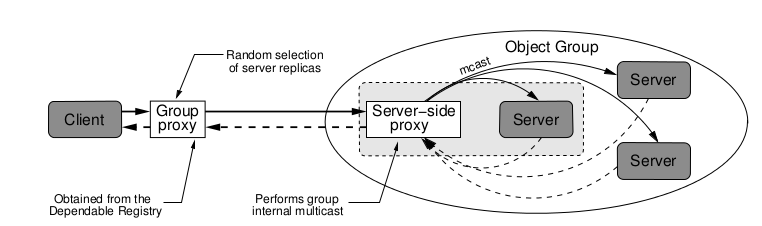
\includegraphics[width=1\textwidth]{arch.png}
  \end{center}
  
  \caption{Overall system architecture}
  \label{path}
\end{wrapfigure}




\end{document} 
